\section{Pivotal trees.}

Let $X$ be a metric space.
A point array $(a_1,\dots,a_n)$ in $X$ together with a choice of a tree with $n$ vertexes labeled by  $(a_1,\dots,a_n)$ and a choice of geodesic $[a_i,a_j]$ for every adjacent pair $(a_i,a_j)$ is called \emph{geodesic tree}.

\hide
\begin{wrapfigure}{r}{15 mm}
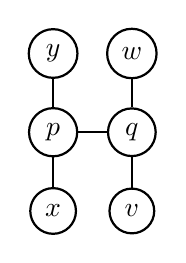
\begin{tikzpicture}[scale=1,
  thick,main node/.style={circle,draw,font=\sffamily\bfseries,minimum size=3mm}]
  \node[main node] (1) at (0,0) {$x$};
  \node[main node] (2) at (0,1){$p$};
  \node[main node] (3) at (0,2){$y$};
  \node[main node] (4) at (1,0) {$v$};
  \node[main node] (5) at (1,1) {$q$};
  \node[main node] (6) at (1,2) {$w$};

  \path[every node/.style={font=\sffamily\small}]
   (1) edge node[above]{}(2)
   (2) edge node[above]{}(3)
   (2) edge node[above]{}(5)
   (4) edge node[above]{}(5)
   (5) edge node[above]{}(6);
\end{tikzpicture}
\end{wrapfigure}
\unhide

For geodesic trees we will use the same notation as for labeled combinatoric tree in square brackets; for example $[p,xy(q,vw)]$ will denote the geodesic tree with with combinatorics as on the diagram. 

Fix a geodeisc dipolar tree $T=[p_1/x_1\dots x_k(p_2/x_{k+1}\dots x_n)]$;
that is, the tree $T$ has two poles $p_1$, $p_2$ and each of the remaining vertexes are adjacent either to $p_1$ or $p_2$;  $x_1,\dots, x_k$ are connected to $p_1$ and $x_{k+1},\dots, x_n$ to $p_2$.

Assume $X$ is a nonnegatively curved Alexandrov space;
in particular the angle is defined for any geodesic hinge. 

A geodesic tree  $\~T=[\~p_1/\~x_1\dots \~x_k(\~p_2/\~x_{k+1}\dots \~x_n)]$ in the Hilbert space $\HH$ will be called \emph{pivotal tree} for $T=[p_1/x_1\dots x_k(p_2/x_{k+1}\dots x_n)]$
if 
\begin{enumerate}[(i)]
\item $|\~p_1-\~p_2|_\HH= |p_1-p_2|_X$,
\item $|\~p_i-\~x_j|_\HH= |p_i-p_j|_X$ for any edge $[p_i,x_j]$ in $T$ and
\item $\measuredangle[\~p_j\,^{\~x_k}_{\~p_i}]_{\HH}=\measuredangle[\~p_j\,^{\~x_k}_{\~p_i}]_X$
for any hinge  $[p_j\,^{x_k}_{\~p_i}]$ in $T$.
\end{enumerate}


\begin{thm}{Rigidity lemma}\label{lem:rigidity}
Let $X$ be a nonnegatively curved Alexandrov space and $T=[p_1/x_1\dots x_k(p_2/x_{k+1}\dots x_n)]$ be geodesic tree in $X$
Suppose  $\~T\zz=[\~p_1/\~x_1\dots \~x_k(\~p_2/\~x_{k+1}\dots \~x_n)]$ is a pivotal tree for  $T$.
Assume that
\[|\~x_i-\~x_j|_\HH\le |x_i-x_j|_X 
\eqlbl{eq:pivotal-comparison}\]
for any pair $(i,j)$ and the convex hull $\~K$ of $\{\~x_1,\dots\~x_n\}$ intersects the line thru $\~p_1$ and $\~p_2$.
Then the equality holds in \ref{eq:pivotal-comparison} for each pair $(i,j)$.
\end{thm}

\parit{Proof.}
Assume that a point $\~z$ on the line $(\~p_1,\~p_2)$ is given.
We can assume that $\~z$ lies on the half-line from $\~p_1$ thru $\~p_2$;
otherwise swap the labels of $\~p_1$ and $\~p_2$.

Denote by $\zeta$ the direction of geodesic $[p_1,p_2]$ at $p_1$. 
Set 
\[z=\gexp_{p_1}(|\~z-\~p_1|\cdot \zeta),\]
where $\gexp_{p_1}$ denotes the gradient exponent at $p_1$; see \cite{AKP-book}. 
By comparison, we have
\begin{align*}
|x_i-z|_X &\le |\~x_i-\~z|_{\RR^2}
\end{align*}
for any $i$.

It remains to apply Kirszbraun rigidity theorem (\ref{thm:kirszbraun-rigid}).
\qeds

Recall that $X$ is a nonnegatively curved Alexandrov space.
Note that by angle comparison, for any $i$ and $j$ we have
\[|\~x_i-\~p_j|_{\HH}\ge |x_i-p_j|_X,\]
where $[\~p_1,\~x_1\dots \~x_k(\~p_2,\~x_{k+1}\dots \~x_n)]$ is a pivotal tree for a geodesic tree  with the vertexes $[p_1,x_1\dots x_k(p_2,x_{k+1}\dots x_n)]$ in $X$.

It follows that the configuration $\~p_1$, $\~p_2$, $\~x_1,\dots\~x_n\in \HH$ satisfies the tree comparison (see Section~\ref{sec:intro}) if 
\[|\~x_i-\~x_j|_{\HH}\ge |x_i-x_j|_X
\eqlbl{eq:tree-comparison}\]
for all pairs $(i,j)$.

Denote by $\~\xi_i$ the direction of the half-plane thru $\~x_i$ with the boundary line $(\~p_1, \~p_2)$.
The direction $\~\xi_i$ lies in the unit sphere normal to the line $(\~p_1, \~p_2)$;
we may assume that the dimension of the sphere is $n-1$.

Note that up to a motion of $\HH$, a pivotal configuration is completely described by the angles $\measuredangle(\~\xi_i,\~\xi_j)$.
Moreover, the distance $|\~x_i-\~x_j|_\HH$ is determined by $\measuredangle(\~\xi_i,\~\xi_j)$ and the function $\measuredangle(\~\xi_i,\~\xi_j)\mapsto |\~x_i-\~x_j|_\HH$ is nondereasing.

Let us denote by $\alpha_{i,j}$ the minimal angle $\measuredangle(\~\xi_i,\~\xi_j)$ in a pivotal configuration such that \ref{eq:tree-comparison} holds, so the inequality \ref{eq:tree-comparison} is equivalent to
\[\measuredangle(\xi_i,\xi_j)\ge \alpha_{i,j}.\]

\begin{thm}{Corollary}\label{cor:|x-x|}
For any geodesic dipolar tree  in a nonnegatively curved Alexandrov space the following conditions hold:
\begin{enumerate}[(a)]
\item For any pair $i$ and $j$, we have
\[\alpha_{i,j}\le \pi.\]
\item For any triple $i$, $j$ and $k$,  we have
\[\alpha_{i,j}+\alpha_{j,k}+\alpha_{k,i}\le 2\cdot\pi.\]
\end{enumerate}
In other words, if $X$ is a nonnegatively curved Alexandrov space then
\begin{enumerate}[(a)]
\item\label{cor:|x-x|:a} For any broken geodesic line $[p_1/x_1(p_2/x_2)]$ in  $X$ there is a pivotal tree $[\~p_1,\~x_1(\~p_2,\~x_2)]$ such that 
\[|\~x_1-\~x_2|_{\HH}\ge |x_1-x_2|_X.\]

\item\label{cor:|x-x|:b} For any geodesic tree $[p_1/x_1x_2(p_2/x_3)]$ in $X$ there is a pivotal tree $[\~p_1/\~x_1\~x_2(\~p_2/\~x_3)]$ such that 
\begin{align*}
|\~x_i-\~x_j|_{\HH}&\ge |x_i-x_j|_X.
\end{align*}
for all $i$ and $j$.
\end{enumerate}

\end{thm}

\parit{Proof; (\ref{cor:|x-x|:a}).}
Consider the pivotal tree $[\~p_1/\~x_1(\~p_2/\~x_2)]$ (which is a polygonal path) with $\measuredangle(\~\xi_1,\~\xi_2)=\pi$.
Note that the points $\~p_1,\~x_1,\~p_2,\~x_2$ are coplanar and the points $\~x_1$ and $\~x_2$ lie on the opposite sides from the line $(\~p_1,\~p_2)$.
It remains to apply the rigidity lemma.

\parit{(\ref{cor:|x-x|:b}).} By \textit{(\ref{cor:|x-x|:a})}, we can assume that \[\alpha_{1,3}+\alpha_{2,3}>\pi.
\eqlbl{sum>pi}\]

Consider the pivotal tree $[\~p_1/\~x_1x_2(\~p_2/\~x_3)]$ which lies in a 3-dimesional subspace in such a way that the points $\~x_1$ and $\~x_2$ lie on the opposite sides from the plane $(\~p_1,\~p_2,\~x_3)$ and 
\begin{align*}
\measuredangle(\~\xi_1,\~\xi_3)&=\alpha_{1,3},
&
\measuredangle(\~\xi_2,\~\xi_3)&=\alpha_{2,3}.
\end{align*}
By \ref{sum>pi}, the convex hull $\~K$ in the rigidity lemma intersects the line $(\~p_1,\~p_2)$.
It remains to apply the lemma.
\qeds

Note that \textit{(\ref{cor:|x-x|:a})} and \textit{(\ref{cor:|x-x|:b})} implies that $X$ satisfies the comparison for the dipolar trees $1(1)$ and $2(1)$ shown on the digram. 
However, the tree comparison for $(1(1))$ follows from the triangle inequality.

\hide
\begin{center}
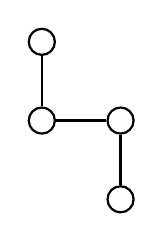
\begin{tikzpicture}[scale=1,
  thick,main node/.style={circle,draw,font=\sffamily\bfseries,minimum size=3mm}]
  \node[main node] (2) at (0,1){};
  \node[main node] (3) at (0,2){};
  \node[main node] (4) at (1,0) {};
  \node[main node] (5) at (1,1) {};
  \path[every node/.style={font=\sffamily\small}]
   (2) edge node[above]{}(3)
   (2) edge node[above]{}(5)
   (4) edge node[above]{}(5);
\end{tikzpicture}
\hskip10mm
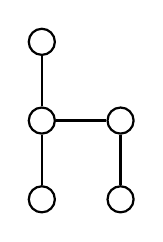
\begin{tikzpicture}[scale=1,
  thick,main node/.style={circle,draw,font=\sffamily\bfseries,minimum size=3mm}]
  \node[main node] (1) at (0,0) {};
  \node[main node] (2) at (0,1){};
  \node[main node] (3) at (0,2){};
  \node[main node] (4) at (1,0) {};
  \node[main node] (5) at (1,1) {};
  

  \path[every node/.style={font=\sffamily\small}]
   (1) edge node[above]{}(2)
   (2) edge node[above]{}(3)
   (2) edge node[above]{}(5)
   (4) edge node[above]{}(5);
\end{tikzpicture}
\end{center}
\unhide

\section{Six point comparison}\label{6-dipole}


\begin{thm}{Theorem}\label{2(2)+3(1)}
Let $X$ be an nonnegatively curved Alexandrov space.
Then for any geodesic 2(2)-tree and any 3(1)-tree (see the diagram) there is a pivotal tree satisfying the tree comparison.


In particular, any nonnegatively curved Alexandrov space satisfies the comparison for 
the bipolar trees 2(2) and 3(1).

\end{thm}

\hide
\begin{center}
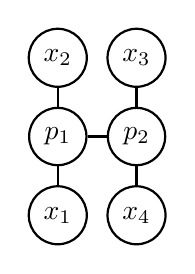
\begin{tikzpicture}[scale=1,
  thick,main node/.style={circle,draw,font=\sffamily\bfseries,minimum size=3mm}]

  \node[main node] (1) at (0,0) {$x_1$};
  \node[main node] (2) at (0,1){$p_1$};
  \node[main node] (3) at (0,2){$x_2$};
  \node[main node] (4) at (1,0) {$x_4$};
  \node[main node] (5) at (1,1) {$p_2$};
  \node[main node] (6) at (1,2) {$x_3$};

  \path[every node/.style={font=\sffamily\small}]
   (1) edge node[above]{}(2)
   (2) edge node[above]{}(3)
   (2) edge node[above]{}(5)
   (4) edge node[above]{}(5)
   (5) edge node[above]{}(6);
\end{tikzpicture}
\hskip10mm
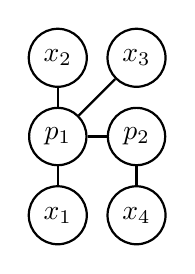
\begin{tikzpicture}[scale=1,
  thick,main node/.style={circle,draw,font=\sffamily\bfseries,minimum size=3mm}]

  \node[main node] (1) at (0,0) {$x_1$};
  \node[main node] (2) at (0,1){$p_1$};
  \node[main node] (3) at (0,2){$x_2$};
  \node[main node] (4) at (1,0) {$x_4$};
  \node[main node] (5) at (1,1) {$p_2$};
  \node[main node] (6) at (1,2) {$x_3$};

  \path[every node/.style={font=\sffamily\small}]
   (1) edge node[above]{}(2)
   (2) edge node[above]{}(3)
   (2) edge node[above]{}(5)
   (2) edge node[above]{}(6)
   (4) edge node[above]{}(5);
\end{tikzpicture}
\end{center}
\unhide



\parit{Proof.} 
The proof in these two cases will be identical.
Fix a geodesic tree $[p_1/x_1x_2(p_2/x_3x_4)]$ or $[p_1/x_1x_2x_3(p_2/x_4)]$.

Recall that $p_1$ and $p_2$ are the poles of the tree and each of remaining vertexes $x_1,x_2, x_3,x_4$ are connected to one of the poles.

Define the values $\{\alpha_{i,j}\}$ for each pair $i,j$ as in the previous section.

Fix a smooth monotonic function $\phi\:\RR\to\RR$ such that $\phi(x)=0$ if $x\ge 0$ and $\phi(x)>0$ if $x<0$.
Consider a configuration of 4 points $\~\xi_1,\~\xi_2,\~\xi_3,\~\xi_4$ in $\SS^3$ which minimize the \emph{energy}
\[E(\~\xi_1,\~\xi_2,\~\xi_3,\~\xi_4)
=
\sum_{i<j}\phi(\measuredangle(\~\xi_i,\~\xi_j)-\alpha_{i,j}).\]

Consider the geodesic graph $\Gamma$ with 4 vertexes $\~\xi_1,\~\xi_2,\~\xi_3,\~\xi_4$ in $\SS^3$, where 
$\~\xi_i$ is adjacent to $\~\xi_j$ if $\measuredangle(\~\xi_i,\~\xi_j)<\alpha_{i,j}$.
If there the comparison does not hold then this graph is not empty.

Note that for any vertex $\~\xi_i$ can not lie in an open hemisphere with all its adjacent vertexes. 
Indeed, if it would be the case then we could move this $\~\xi_i$ increasing the distances to all its adjacent vertexes.
Along this move the energy decreases which is not possible.

Note that by Corollary \ref{cor:|x-x|}, degree of any vertex is at least 2.
Indeed existence of a vertex of degree 1 contradicts \ref{cor:|x-x|}\textit{\ref{cor:|x-x|:a}} and existence of a vertex of degree 0 contradicts \ref{cor:|x-x|}\textit{\ref{cor:|x-x|:b}}.

Therefore we are left with the following three graphs.

\hide
\begin{center}
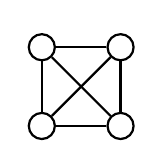
\begin{tikzpicture}[scale=1,
  thick,main node/.style={circle,draw,font=\sffamily\bfseries,minimum size=3mm}]

  \node[main node] (1) at (0,0) {};
  \node[main node] (2) at (0,1){};
  \node[main node] (3) at (1,1){};
  \node[main node] (4) at (1,0) {};

  \path[every node/.style={font=\sffamily\small}]
   (1) edge node[above]{}(2)
   (2) edge node[above]{}(3)
   (2) edge node[above]{}(4)
   (3) edge node[above]{}(1)
   (3) edge node[above]{}(4)
   (1) edge node[above]{}(4);
\end{tikzpicture}
\hskip10mm
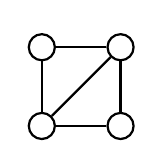
\begin{tikzpicture}[scale=1,
  thick,main node/.style={circle,draw,font=\sffamily\bfseries,minimum size=3mm}]

  \node[main node] (1) at (0,0) {};
  \node[main node] (2) at (0,1){};
  \node[main node] (3) at (1,1){};
  \node[main node] (4) at (1,0) {};

  \path[every node/.style={font=\sffamily\small}]
   (1) edge node[above]{}(2)
   (2) edge node[above]{}(3)
   (3) edge node[above]{}(1)
   (3) edge node[above]{}(4)
   (1) edge node[above]{}(4);
\end{tikzpicture}
\hskip10mm
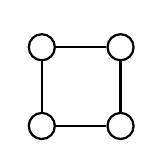
\begin{tikzpicture}[scale=1,
  thick,main node/.style={circle,draw,font=\sffamily\bfseries,minimum size=3mm}]

  \node[main node] (1) at (0,0) {};
  \node[main node] (2) at (0,1){};
  \node[main node] (3) at (1,1){};
  \node[main node] (4) at (1,0) {};

  \path[every node/.style={font=\sffamily\small}]
   (1) edge node[above]{}(2)
   (2) edge node[above]{}(3)
   (3) edge node[above]{}(4)
   (1) edge node[above]{}(4);
\end{tikzpicture}
\end{center}
\unhide

The 6-edege case (that is, the complete graph with 4 vertexes) can not appear by the rigidity lemma (\ref{lem:rigidity}).

To do the remaining two cases, note that since energy is minimal, the angle between the edges at every vertex of degree 2 of $\Gamma$ has to be $\pi$. 
That is, the pair of edges at such vertex forms a geodesic.

Consider the 5-edge graph on the diagram.
By the observation above the two triangles in the graph forms an equator.
The latter contradicts Corollary \ref{cor:|x-x|}\textit{\ref{cor:|x-x|:b}}.

For the 4-edge graph,
by the same observation we have 4 points lie on the equator; 
moving one pair to north pole and the other to south pole will increase all 4 edges, a contradiction.
\qeds

